The goal of the experiment was measure the performance change in a maneuvering task using a predictor display based on image transformation on a real ROV. The participants were given a modified "peg-in-hole" task, where the peg was mounted on a remotely controlled ground vehicle and the holes were rectangular holes in a wooden box.

%A camera was mounted on the ROV such that the operator could see the peg and holes. The goal of the experiment was to measure the operator's navigational performance difference using two different display types. Both displays would use the same fixed delay, but the second would use predictive technology to visualize instant robot responses. The first display would contain a delayed video feed from an ROV while the other display used predictive visualization with the same delay. The participants were given a task of maneuvering the UGV to three specific locations as many times as possible in the course of 90 seconds.

\section{Participants}

The participants were voluntary selected from the NTNU Department of Mechanical and Industrial Engineering. A total of 58 participants performed the experiment whereas the first one were excluded from the data foundation. This was due to lack of information that became evident during the first trial. This information were given to the other 57 participants. None of the participants had any earlier experience with predictive displays.

35.1\% of the participants were female and the total group had an average age of 24.7 years with an standard deviation of 1.45. 100\% of the group reported that they use a computer on a daily basis. When asked how often he or she play video games (computer or console), the distribution were as follows: daily 4\%, weekly 26\%, monthly 14\%, yearly 30\% and never 26\%.

\section{Experimental design}
\todo[inline]{
- robot

- controlling (can not see robot)

- delay

- task

- testing Fitt's law

- layout of the button case
}

\begin{figure}[h!]
    \centering
    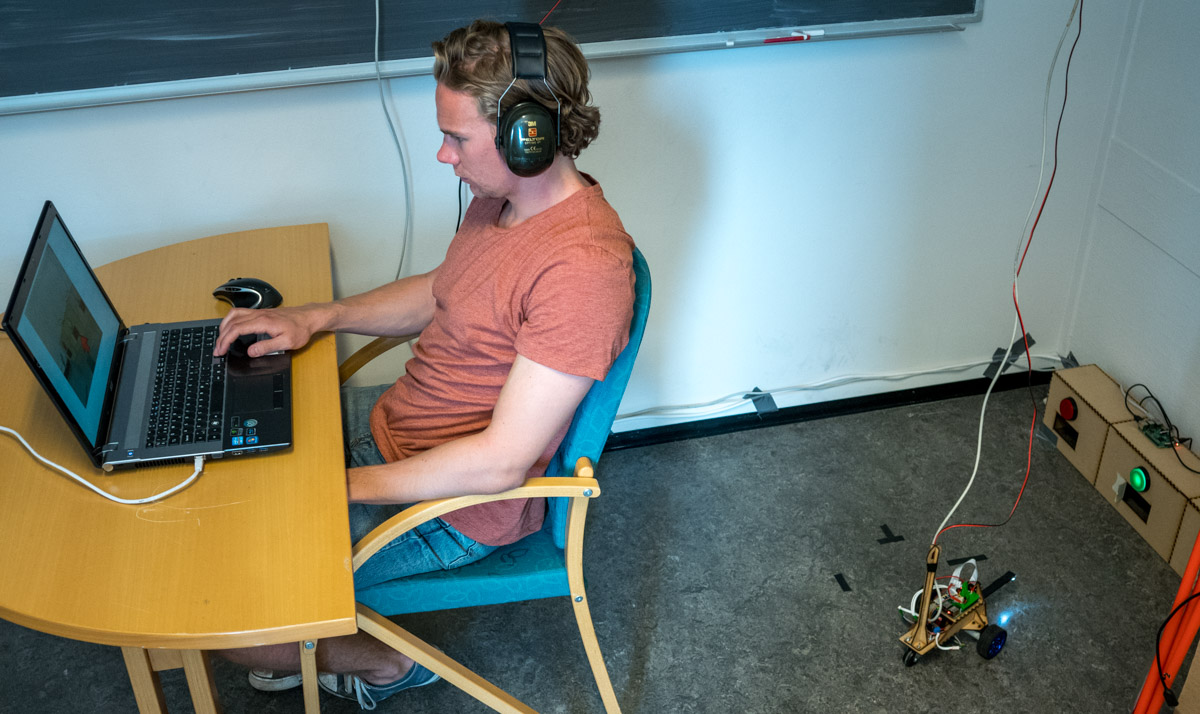
\includegraphics[width=0.9\textwidth]{setup-2}
    \caption{Experimental setup.}
    \label{expsetup}
\end{figure}

\figref{expsetup} shows an overview of the experimental setup. A 17 inch laptop running with a 2.3GHz Intel Core i7-3610QM CPU and Windows 10 were used as the operator's control device. This was connected to the ROV through a direct Ethernet connection. The ROV, \figref{setup3}, was a three wheeled robot running a Raspberry Pi 3 Model B+. Two of the wheels where connected to each their DC-motor while the third one was a caster wheel for support. The ROV was equipped with a forward facing Raspberry Pi Camera V2 with a wide angle lens attached. The robot were running the eduROV software outlined in chapter \ref{chpEdurov}. This software was responsible for serving the control interface, handling commands, logging experiment data and adding the desired latency to the communication.

One by one, i random order, the round LED would light up. The operator was then tasked to maneuver the ROV such that the black peg would go inside the corresponding hole. A light sensor inside the hole would register this as a \emph{hit} which would cause the LED to turn off, and one of the other two would light up. The participant were told to make as many \emph{hits} as possible in the course of 90 seconds.

The participant would repeat this task a total of three times, using three different displays / conditions. The order of these conditions followed a 3x3 Latin Square Design, to eliminate the order effect. Condition one had a total delay of 700 ms which includes the inherent delay of the system 250ms, plus the added delay of 450 ms. Condition two had the same delay as condition one, but with the predictive display in effect. The third condition had no added delay and only the inherent delay of 250ms. No predictive technology were used in the third condition.

\begin{figure}[h!]
    \centering
    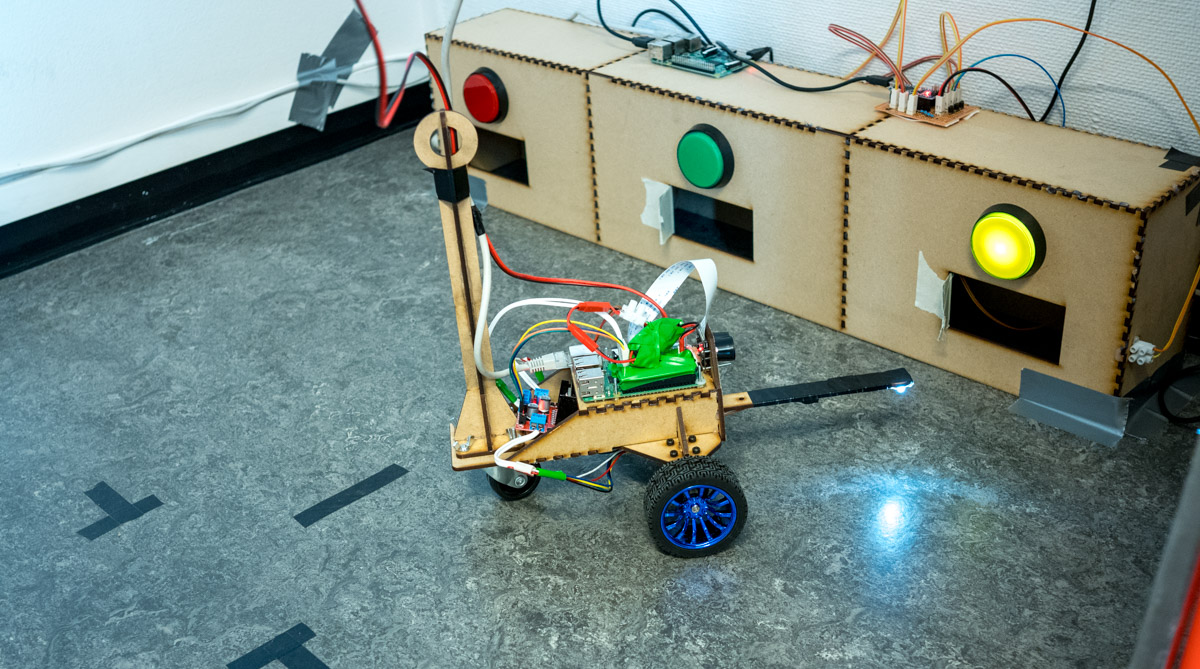
\includegraphics[width=0.9\textwidth]{setup-3}
    \caption{Three wheeled robot used in experiment.}
    \label{setup3}
\end{figure}



keep it simple to reduce variance i results, but complex enough that the effects of video delay would be noticeable (and predictor could help)

other experiments where "task completion time" is used may have been limited by the speed of the robot / got stuck in the walls

"human subject experiments"

avoid ceiling effects (to slow robot/to easy tasks)

robot software, electronics, equipment, 2 DOF, rotation and forward/backward

relevant delay for wireless high definition low cost solution, or very long range (digital), what are the delays


\section{Procedure}
\todo[inline]{
- groups

- what information were they given

- training

- time of experiment

- reposition of robot

- demographics at start

- answered survey for each exp
}

running a warmup where the user familiarizes himself with the input device and kinematics of the robot

\citep{Lu2018} "Condition order followed a 3x3 Latin-Square Design, so as to eliminate the order effect"

"delay conditions were presented to the participants in a counterbalanced order to control for possible learning effects."

info: goal of exp, be awera of wall, rocker wheel, information page

were NOT told that one of the displays is a predictor displays


\section{Data recording}
\todo[inline]{
- Hits / Score at time

- camera

- NASA TLX

- keypresses

- surveys

- SQLite
}

"(Three) metrics are used to quantify performance;"

"steering control effort is monitored to assess drivability" (TLX)


\section{Performance analysis}
\todo[inline]{
- how was the performance quantified

- normalization (Yip2011)

- t-test when comparing two displays, ANOVA when comparing three

- t-test: scipy.stats.ttest\_rel

- cohens d: appendix

- \citep{Rachmielowski2010} and \citep{Lovi2014} Normalized data the same way

- APA style

- effect size

- paried sample t-test

- T value means that they are 4 times more different from each other than they are within
}
